% !TeX encoding = UTF-8
% !TeX spellcheck = ru_RU
\documentclass[12pt,a4paper]{article}

\usepackage[T2A]{fontenc}
\usepackage[utf8]{inputenc}
\usepackage[russian]{babel}
\usepackage{amsmath,amssymb}
\usepackage{graphicx}
\usepackage{float}
\usepackage{array}
\usepackage{booktabs}
\usepackage{url}
\usepackage{kprj}

\setcounter{secnumdepth}{3}
\setcontentsname{СОДЕРЖАНИЕ}
\setrefsname{Список литературы}
\equationnumbering{section}
\figurenumbering{section}
\SkipContentsbreak

\ifpdftex
\usepackage[unicode=true]{hyperref}
\hypersetup{
  pdfpagemode=UseNone,
  pdfstartview=FitH,
  colorlinks=true,
  linkcolor=black,
  citecolor=black,
  urlcolor=black
}
\fi

\ifpdftex
\DeclareGraphicsExtensions{.pdf,.png,.jpg}
\else
\DeclareGraphicsExtensions{.eps}
\fi

\renewcommand{\arraystretch}{1.12}
\sloppy

\NIR
\makeatletter
\makeatother

\Ministry{Министерство науки и высшего образования Российской Федерации}
\BMSTU{Федеральное государственное автономное образовательное\\
учреждение высшего образования\\
\al{}Московский государственный технический университет\\
имени Н.\,Э.~Баумана (национальный\\
исследовательский университет)\ar{}\\
(МГТУ им. Н.Э.~Баумана)}

\title{Подход Large Neighborhood Search в задаче 3D Bin Packing}
\authorfull{Иртюга Илья Владимирович}
\author{Иртюга И. В.}
\workyear{2026}
\group{ФН12-81Б}
\faculty{фундаментальных наук}
\facultyshort{ФН}
\chair{математического моделирования}
\chief{Фетисов Д. А.}
\trend{исследовательская}
\themesource{кафедра}

\begin{document}

\maketitle
\tableofcontents
\newpage

\section{Введение}

Задача трёхмерной упаковки прямоугольных объектов в ограниченный контейнер относится к классу сложных комбинаторных задач и имеет прямое прикладное значение для складской логистики, паллетизации и транспортировки грузов~[1]. В практических приложениях важно не просто разместить как можно больше коробок, но и соблюдать ограничения по массе, устойчивости, ориентации и хрупкости товара.

В рассматриваемом проекте исследуется single-pallet постановка задачи 3D Bin Packing. Для неё уже была выполнена курсовая работа, в которой кратко сравнивались алгоритмы решения. В настоящей НИР внимание сосредоточено только на одном методе --- \textit{Large Neighborhood Search} (LNS). Именно этот подход показывает лучшие результаты на общих наборах данных проекта по итоговой метрике качества.

\textbf{Цель работы} --- исследовать применение подхода Large Neighborhood Search к задаче 3D Bin Packing и объяснить, почему данный метод превосходит базовый greedy-алгоритм.

\textbf{Для достижения цели решаются следующие задачи:}
\begin{enumerate}
  \item формализовать постановку задачи и используемую метрику качества;
  \item кратко описать greedy как базовый метод;
  \item подробно разобрать структуру и параметры LNS-алгоритма;
  \item рассмотреть реализацию LNS в проекте;
  \item сравнить LNS и greedy по имеющимся экспериментальным результатам;
  \item сформулировать выводы о достоинствах и ограничениях подхода.
\end{enumerate}

\textbf{Объект исследования} --- алгоритмы укладки прямоугольных коробок на паллету.

\textbf{Предмет исследования} --- метаэвристический подход Large Neighborhood Search и его практическое применение к задаче 3D Bin Packing.

\section{Постановка задачи}

Каждая задача в проекте задаётся в формате JSON и включает описание одной паллеты и набора типов коробок. Для паллеты указываются длина, ширина, максимальная высота укладки и допустимая масса. Для каждого типа коробки задаются размеры, масса, количество экземпляров и логические признаки \texttt{strict\_upright}, \texttt{fragile}, \texttt{stackable}.

Цель алгоритма состоит в том, чтобы построить допустимую укладку коробок внутри паллеты. При этом должны выполняться следующие ограничения:
\begin{enumerate}
  \item каждая коробка целиком находится внутри габаритов паллеты;
  \item коробки не пересекаются по объёму;
  \item суммарная масса не превышает ограничение паллеты;
  \item для коробок с признаком \texttt{strict\_upright} запрещён поворот, меняющий исходную высоту;
  \item если коробка расположена выше пола паллеты, не менее 60\% площади её основания должно иметь опору;
  \item тяжёлые коробки не должны располагаться над хрупкими без штрафа по метрике.
\end{enumerate}

Качество решения определяется формулой
\[
\text{score} =
0.50 \cdot U_{\text{vol}} +
0.30 \cdot C_{\text{items}} +
0.10 \cdot F_{\text{frag}} +
0.10 \cdot T_{\text{time}},
\]
где $U_{\text{vol}}$ --- коэффициент заполнения объёма паллеты, $C_{\text{items}}$ --- доля размещённых объектов, $F_{\text{frag}}$ --- оценка по хрупкости, $T_{\text{time}}$ --- временной балл.

Из этой формулы видно, что главными компонентами качества являются заполнение контейнера и полнота размещения. Именно поэтому для рассматриваемой задачи особенно важен метод, умеющий улучшать уже найденную укладку, а не только быстро строить первое допустимое решение.

\subsection{Greedy как базовый метод}

Жадный алгоритм используется как baseline и как основа для старта LNS. Он разворачивает количества коробок в последовательность экземпляров, сортирует их по приоритету и затем поочерёдно пытается разместить каждый объект в допустимую позицию. В качестве кандидатов используются \textit{extreme points}, а положение коробки уточняется по схеме ``gravity drop'', то есть с опусканием на минимально возможную высоту.

Преимущество greedy-подхода состоит в скорости и простоте. Недостаток состоит в локальности: если неудачное размещение выполнено на раннем шаге, алгоритм уже не может вернуться назад и перестроить структуру укладки. В результате ухудшается использование свободного пространства и уменьшается доля размещённых коробок.

\section{Метод Large Neighborhood Search}

\subsection{Общая идея LNS}

Подход Large Neighborhood Search относится к метаэвристикам крупноокрестностного поиска~[2]. Его основная идея состоит в том, что решение улучшается не малыми локальными перестановками, а за счёт разрушения значимой части текущей конфигурации и последующего восстановления этой части более удачным образом.

Для задач упаковки такой подход особенно естественен. Если несколько коробок были неудачно размещены в начале, они могут заблокировать большой объём пространства. Тогда локальная правка одной позиции уже не помогает, а частичная перестройка решения позволяет освободить полезные области паллеты и перераспределить объекты более компактно.

\subsection{Этапы работы алгоритма}

В проекте LNS работает по следующей схеме:
\begin{enumerate}
  \item строится начальное жадное решение;
  \item выбирается часть текущей укладки, которая удаляется;
  \item образовавшееся частичное решение стабилизируется;
  \item удалённые и непомещённые объекты заново вставляются процедурой восстановления;
  \item новое решение оценивается и либо принимается, либо отвергается.
\end{enumerate}

Такая структура позволяет сочетать преимущества двух подходов: greedy быстро даёт допустимый старт, а LNS затем выходит за пределы локально жадного выбора.

\subsection{Разрушение и восстановление решения}

На этапе разрушения из текущей укладки удаляется часть коробок. В реализации проекта используются разные destroy-эвристики: случайное удаление, удаление верхних коробок, удаление кластера около случайной коробки, удаление элементов, связанных с нарушениями хрупкости, и полный рестарт. Число удаляемых объектов зависит от текущего размера укладки и параметров конфигурации.

После destroy-фазы вызывается стабилизация частичного решения: если какие-то коробки потеряли опору и стали ``зависшими'', они тоже удаляются. Это делает промежуточное состояние геометрически согласованным.

Далее запускается этап repair. В текущей реализации он основан на beam search. Алгоритм рассматривает несколько лучших частичных состояний, для каждого перебирает допустимые повороты и extreme points, проверяет пересечения, опору и ограничения по хрупкости, после чего оставляет наиболее перспективные варианты для дальнейшего расширения. Благодаря этому восстановление оказывается заметно сильнее, чем одношаговый greedy-выбор.

\subsection{Критерий принятия решения}

После восстановления укладка оценивается той же целевой функцией, что и финальный ответ. Если новое решение лучше лучшего найденного ранее, оно сохраняется. Кроме того, в проекте используется simulated annealing: часть ухудшений может быть принята как текущее рабочее состояние с вероятностью, зависящей от температуры. Это позволяет алгоритму выходить из локальных максимумов.

Если на протяжении нескольких итераций улучшения не происходит, включается механизм перезапуска поиска. Он формирует новую рабочую точку из лучшего найденного решения, но с другой перестановкой очереди объектов. Такая комбинация LNS и управляемых рестартов повышает устойчивость метода.

\section{Реализация LNS в проекте}

\subsection{Общая структура реализации}

Реализация LNS тесно связана с greedy-алгоритмом: используются общие процедуры генерации допустимых поворотов, проверки опоры, хрупкости и пересечений, а также пространственная структура данных, ускоряющая геометрические проверки. Поэтому LNS не дублирует базовую геометрию, а опирается на уже согласованные механизмы.

Основные смысловые блоки реализации таковы:
\begin{enumerate}
  \item конфигурации параметров алгоритма;
  \item процедура построения начального решения;
  \item функции вычисления итоговой и частичной оценки;
  \item набор destroy-эвристик;
  \item процедуры восстановления решения;
  \item главный цикл оптимизации.
\end{enumerate}

\subsection{Начальное решение}

Начальное решение строится жадно, но не единственным запуском. Сначала применяется базовая сортировка товаров, затем выполняется несколько детерминированных вариантов упорядочивания, а после этого --- серия случайных greedy-рестартов в пределах выделенного временного бюджета. Итогом фазы становится лучший жадный результат, найденный на старте.

Это важная особенность реализации: LNS стартует не с произвольной укладки, а с уже усиленного greedy-решения. Тем самым сокращается расстояние до качественного ответа и повышается эффективность последующего поиска.

\subsection{Destroy-эвристики и стабилизация}

В реализации используются несколько destroy-операторов. Для single-pallet постановки особенно важны следующие идеи:
\begin{enumerate}
  \item удаление верхних коробок позволяет перестроить верхние уровни и лучше использовать высоту;
  \item удаление кластера позволяет локально перепланировать плотную область;
  \item удаление коробок, близких по объёму к непомещённым, освобождает место для более выгодной перестановки;
  \item полный рестарт помогает выйти из тупиковой конфигурации.
\end{enumerate}

После разрушения вызывается процедура стабилизации, которая каскадно удаляет коробки без достаточной опоры. Благодаря этому beam search всегда восстанавливает уже согласованное частичное решение.

\subsection{Процедура repair}

Процедура восстановления является центральной частью всей реализации. Её основу составляет beam search. Алгоритм хранит не полные копии укладки, а только изменения относительно фиксированной части, то есть \textit{delta-state}. Это уменьшает накладные расходы при поиске.

Для каждого луча beam search вычисляется частичная оценка
\[
\text{partial\_score} =
0.50 \cdot U_{\text{vol}} +
0.30 \cdot C_{\text{items}} -
0.005 \cdot n_{\text{frag\_viol}},
\]
которая ориентирует поиск на лучшее заполнение объёма и большее число размещённых объектов при умеренном штрафе за проблемы хрупкости.

Дополнительно восстановление выполняется не один раз: очередь рассматриваемых объектов несколько раз случайно переставляется, и из нескольких запусков выбирается лучший результат. Таким образом, repair сочетает направленный поиск и стохастическое разнообразие.

\subsection{Ключевые параметры}

Наиболее важные параметры основной конфигурации LNS приведены в таблице~\ref{tab:cfg}.

\begin{table}[H]
\small
\centering
\caption{Ключевые параметры основной конфигурации LNS}
\label{tab:cfg}
\begin{tabular}{>{\raggedright\arraybackslash}p{0.31\textwidth}cc>{\raggedright\arraybackslash}p{0.30\textwidth}}
\toprule
\textbf{Параметр} & \textbf{Значение} & \textbf{Блок} & \textbf{Смысл} \\
\midrule
\texttt{time\_budget\_s} & 4.8 & поиск & общий бюджет времени \\
\texttt{greedy\_phase\_s} & 1.5 & старт & бюджет на greedy-рестарты \\
\texttt{destroy\_k\_fraction} & 0.15 & destroy & доля удаляемых коробок \\
\texttt{beam\_width} & 8 & repair & число лучей beam search \\
\texttt{repair\_queue\_limit} & 50 & repair & размер очереди на восстановление \\
\texttt{repair\_restarts} & 2 & repair & число дополнительных запусков восстановления \\
\texttt{early\_stop\_patience} & 25 & управление & порог остановки по застою \\
\texttt{ils\_kicks} & 5 & управление & число перезапусков поиска \\
\texttt{sa\_initial\_temp} & 0.015 & приём & стартовая температура \\
\texttt{sa\_cooling\_rate} & 0.92 & приём & коэффициент охлаждения \\
\bottomrule
\end{tabular}
\end{table}

\section{Экспериментальное сравнение LNS и Greedy}

\subsection{Данные для сравнения}

Для анализа использованы сохранённые результаты вычислительных экспериментов для greedy и LNS. Рассматриваются три общих набора задач:
\begin{enumerate}
  \item \texttt{dataset\_100.json} --- 100 задач;
  \item \texttt{dataset\_200\_2.json} --- 200 задач;
  \item \texttt{dataset\_benchmark.json} --- 200 задач.
\end{enumerate}

Для построения графиков в проект НИР включён воспроизводимый скрипт, который обрабатывает сохранённые результаты и формирует сводные рисунки и таблицы.

\subsection{Итоговый score}

Средние значения итогового \texttt{score} приведены в таблице~\ref{tab:score}.

\begin{table}[H]
\centering
\caption{Сравнение LNS и greedy по итоговому score}
\label{tab:score}
\begin{tabular}{lcccc}
\toprule
\textbf{Набор} & \textbf{Greedy} & \textbf{LNS} & $\Delta$ & \textbf{Преимущество LNS} \\
\midrule
\texttt{dataset\_100} & 0.684 & 0.711 & +0.027 & устойчивое \\
\texttt{dataset\_200\_2} & 0.712 & 0.743 & +0.031 & устойчивое \\
\texttt{dataset\_benchmark} & 0.655 & 0.730 & +0.075 & сильное \\
\bottomrule
\end{tabular}
\end{table}

Во всех трёх случаях LNS превосходит базовый greedy-алгоритм. Особенно заметен выигрыш на \texttt{dataset\_benchmark}, где задачи сложнее и пространство возможных перестроек богаче. Это подтверждает, что крупноокрестностный поиск особенно полезен тогда, когда одной жадной проходки уже недостаточно.

\begin{figure}[H]
  \centering
  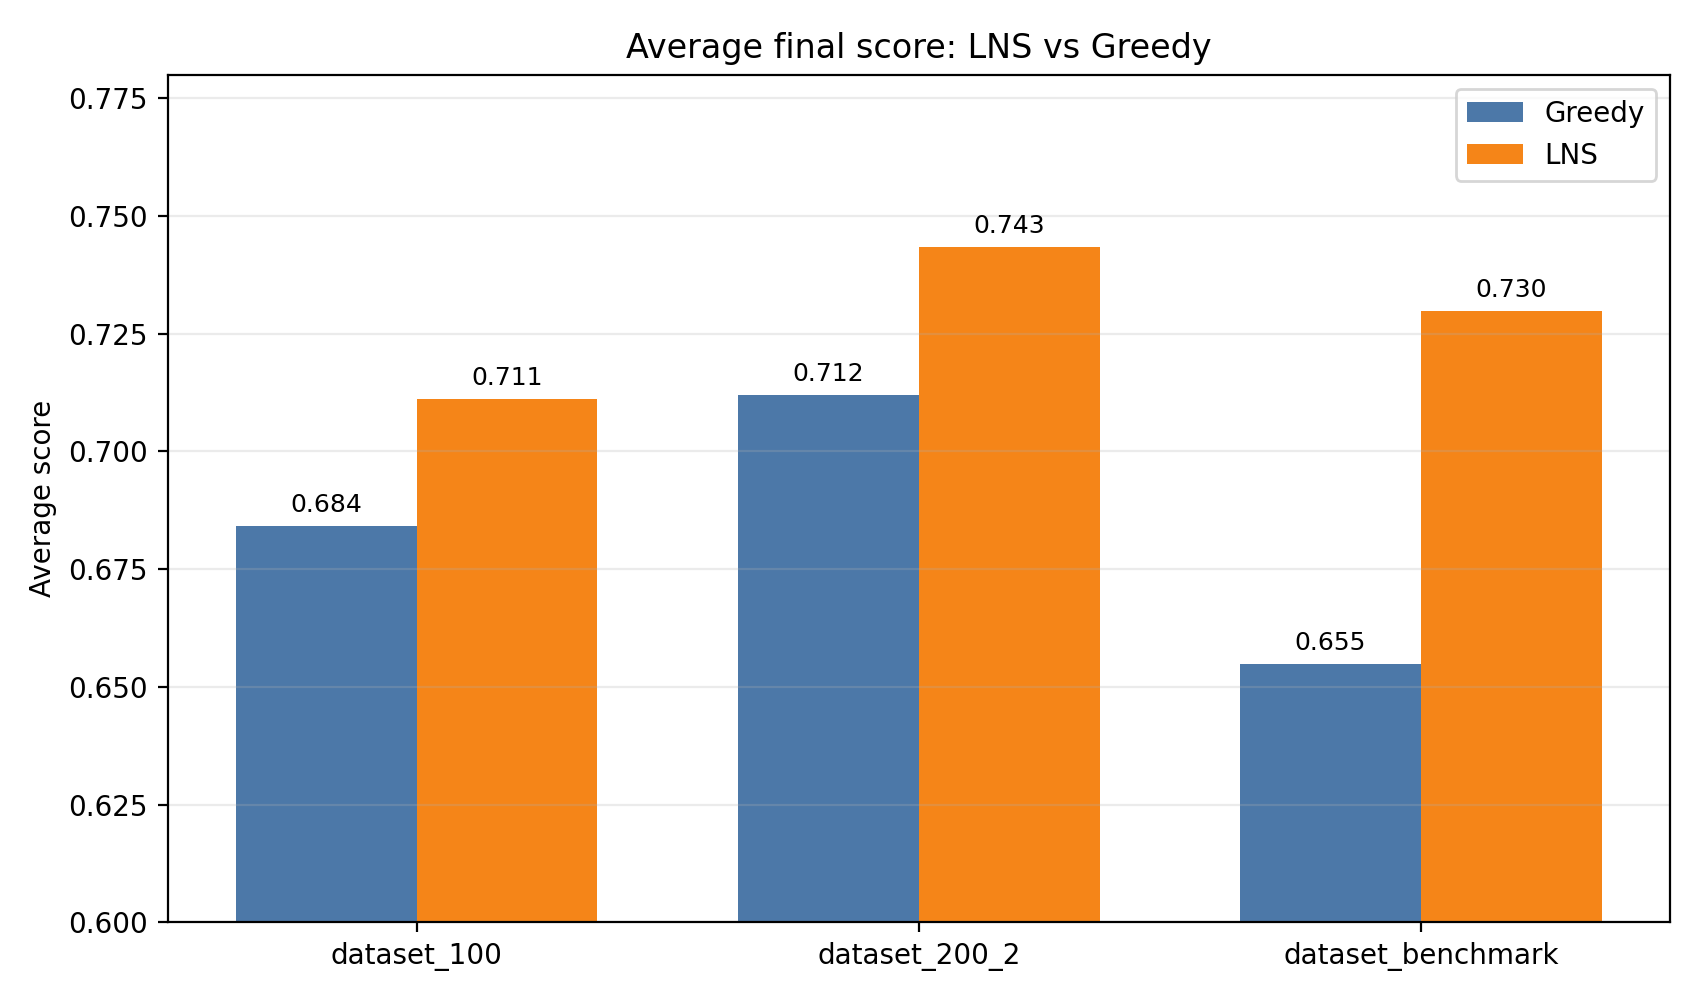
\includegraphics[width=0.84\textwidth]{images/lns_vs_greedy_score.png}
  \caption{Средний итоговый score для LNS и greedy}
\end{figure}

\subsection{Компоненты метрики}

Для понимания причин превосходства полезно посмотреть на компоненты метрики. Наиболее показателен набор \texttt{dataset\_benchmark.json}; результаты приведены в таблице~\ref{tab:bench}.

\begin{table}[H]
\centering
\caption{Компоненты метрики на \texttt{dataset\_benchmark}}
\label{tab:bench}
\begin{tabular}{lccccc}
\toprule
\textbf{Метод} & \textbf{Score} & \textbf{Volume} & \textbf{Coverage} & \textbf{Fragility} & \textbf{Time} \\
\midrule
Greedy & 0.6549 & 0.6155 & 0.4906 & 1.0000 & 1.0000 \\
LNS & 0.7298 & 0.7172 & 0.6036 & 0.9833 & 0.9175 \\
\bottomrule
\end{tabular}
\end{table}

LNS немного уступает greedy по времени и совсем незначительно по компоненте хрупкости, однако существенно выигрывает по двум главным составляющим: использованию объёма и доле размещённых объектов. Именно эти улучшения и дают основной прирост итогового балла.

\begin{figure}[H]
  \centering
  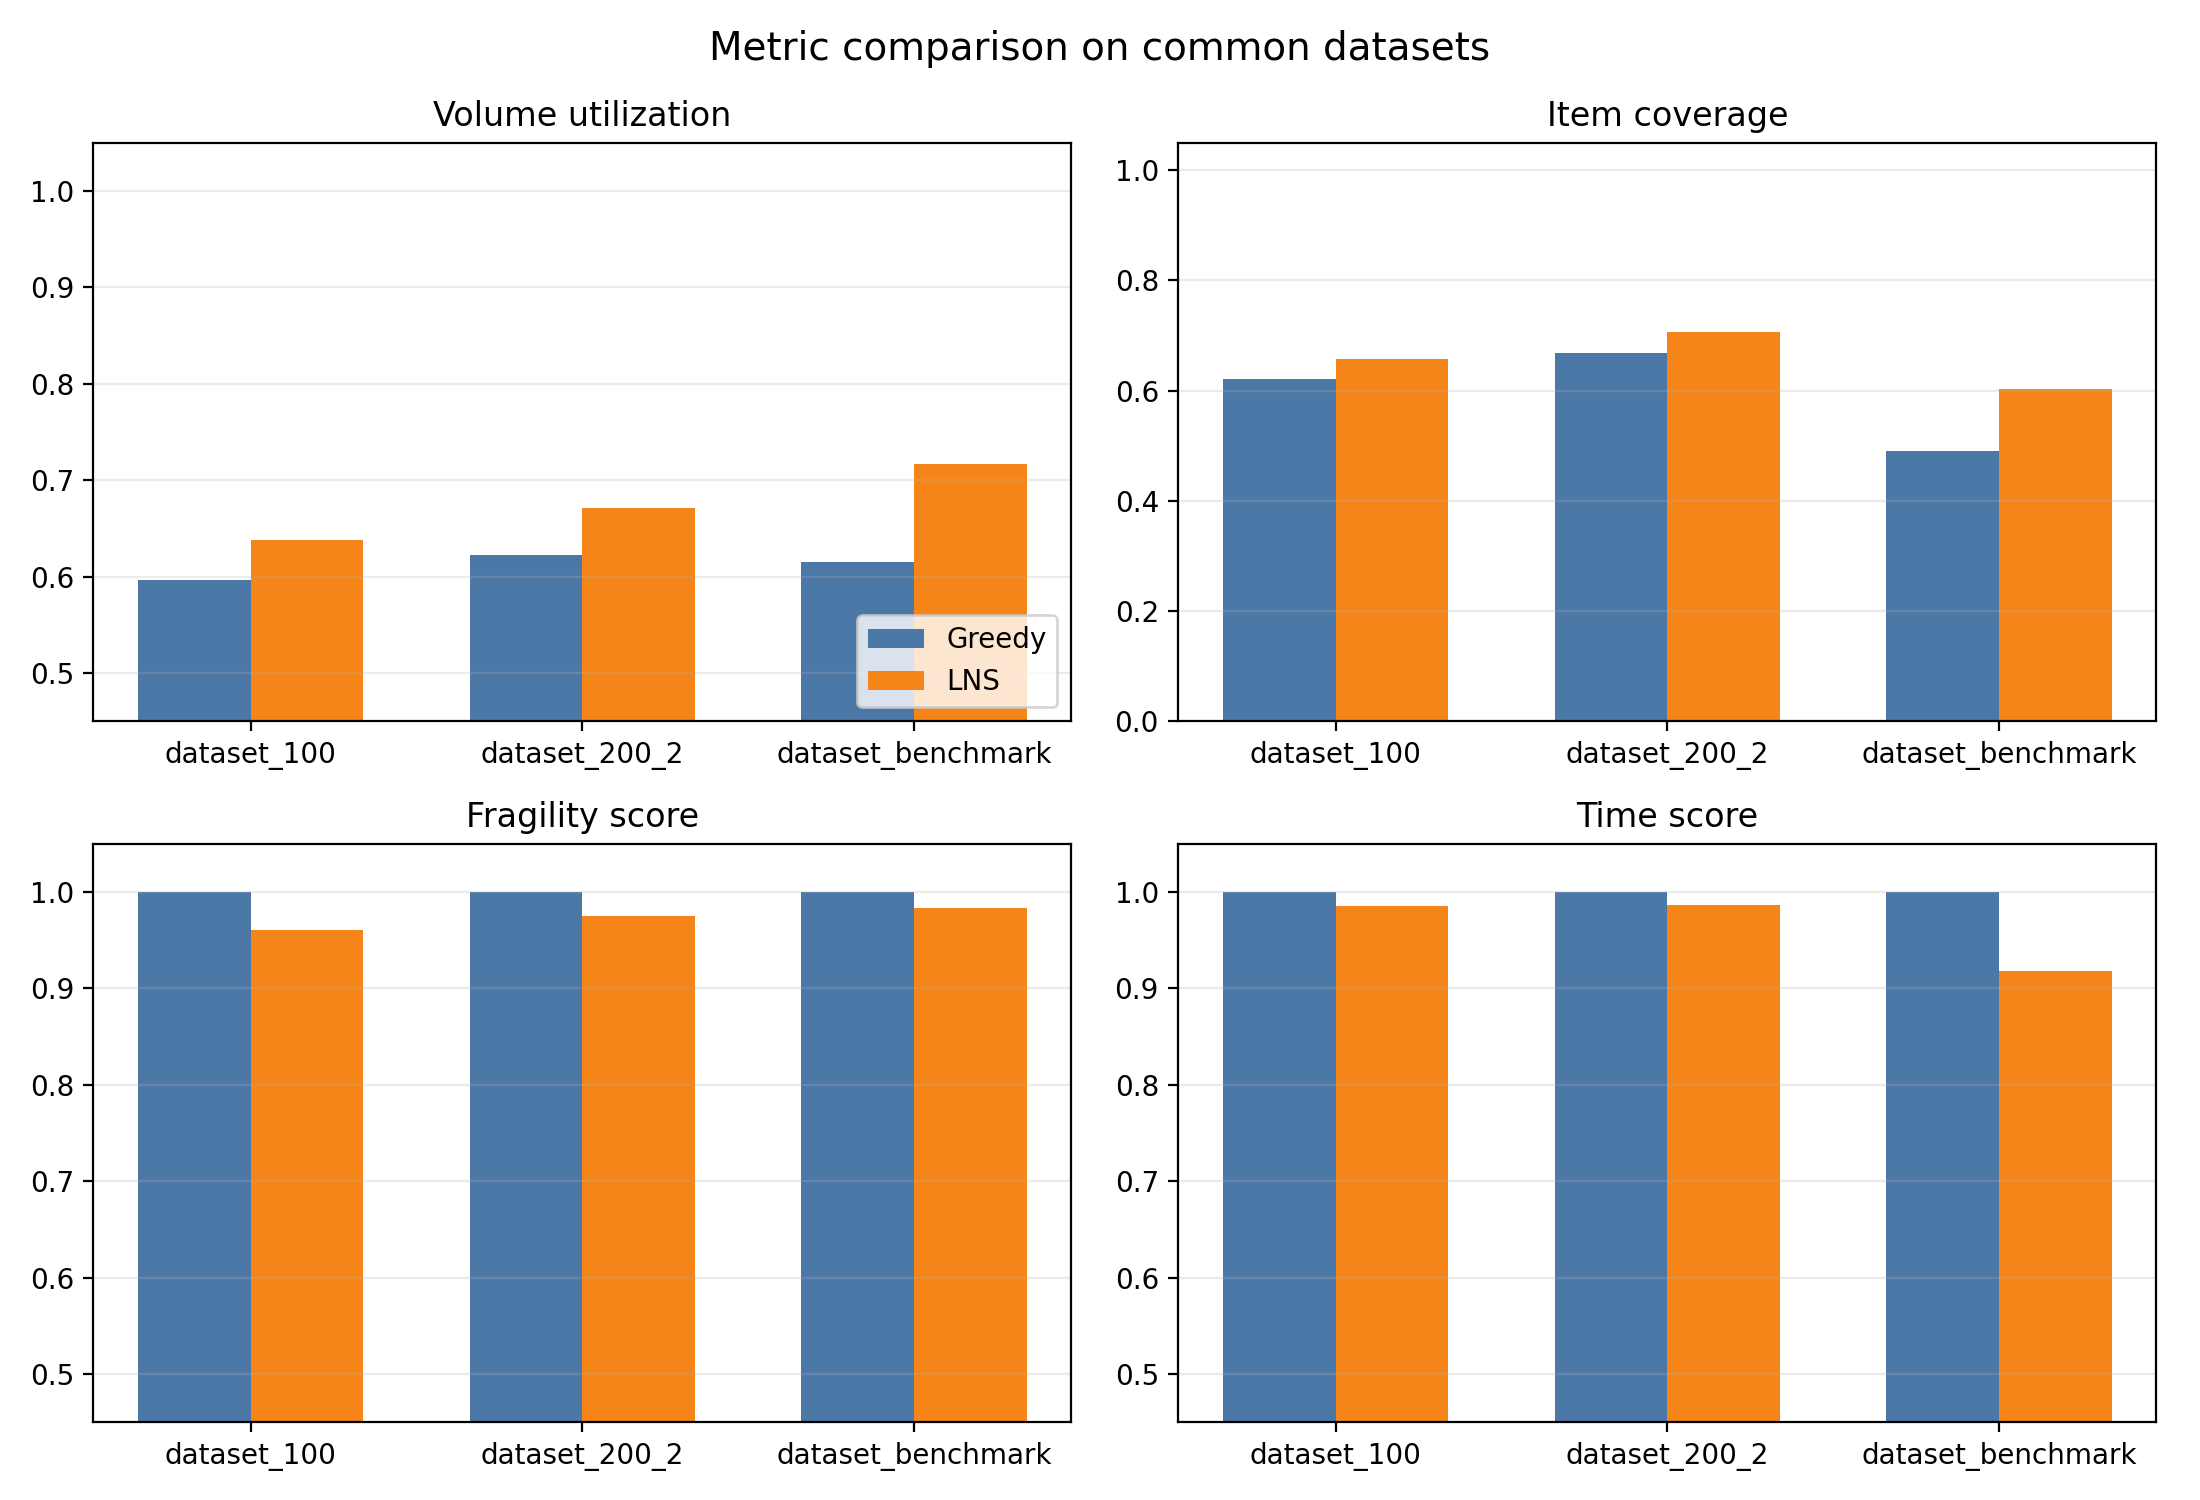
\includegraphics[width=0.93\textwidth]{images/lns_vs_greedy_metrics.png}
  \caption{Сравнение компонент метрики на общих наборах}
\end{figure}

\subsection{Интерпретация результатов}

Преимущество LNS над greedy объясняется структурно:
\begin{enumerate}
  \item greedy принимает решения только один раз, а LNS умеет пересматривать уже построенную укладку;
  \item частичное разрушение решения помогает убрать последствия плохого раннего выбора;
  \item beam search на этапе repair сильнее использует освободившееся пространство;
  \item simulated annealing позволяет не застревать в локально хороших, но глобально слабых конфигурациях.
\end{enumerate}

Именно поэтому LNS лучше заполняет паллету и чаще размещает больше коробок, чем baseline. При этом потеря по времени оказывается умеренной: среднее время решения растёт, но остаётся в разумных границах для заданной метрики.

\section{Выводы}

В работе была рассмотрена single-pallet постановка задачи 3D Bin Packing и подробно исследован подход Large Neighborhood Search. Показано, что данная реализация строится поверх жадного начального решения и усиливает его за счёт повторных перестроек укладки, направленных destroy-операторов, beam-search восстановления и критерия принятия на основе simulated annealing.

Сравнение с greedy-алгоритмом показало, что LNS стабильно выигрывает по итоговому score на всех общих наборах данных проекта. Главная причина состоит в том, что метод лучше использует свободный объём паллеты и размещает большую долю коробок. Таким образом, LNS оказывается наиболее эффективным подходом для данной постановки задачи.

Ограничения метода связаны прежде всего с большей сложностью настройки и более высоким временем работы по сравнению с greedy. Тем не менее в рамках рассматриваемого проекта этот рост времени оказывается оправданным, поскольку улучшение ключевых компонент метрики значительно перекрывает потери по временной составляющей.

\newpage
\section{Список литературы}

\begin{enumerate}
  \item Martello S., Pisinger D., Vigo D. The Three-Dimensional Bin Packing Problem // \textit{Operations Research}. 2000. Vol. 48. No. 2. P. 256--267. DOI: \url{https://doi.org/10.1287/opre.48.2.256.12386}.

  \item Pisinger D., R{\o}pke S. Large Neighborhood Search // \textit{Handbook of Metaheuristics}. 2nd ed. Springer, 2010. P. 399--420.

  \item Faroe O., Pisinger D., Zachariasen M. Guided Local Search for the Three-Dimensional Bin-Packing Problem // \textit{INFORMS Journal on Computing}. 2003. Vol. 15. No. 3. P. 267--283.

  \item Статья из журнала Института системного анализа РАН [Электронный ресурс]. URL: \url{http://www.isa.ru/aidt/2016-03/31_43.pdf} (дата обращения: 27.04.2026).
\end{enumerate}

\end{document}
